\documentclass[../weekly]{subfiles}

\begin{document}

\letAswatheertha

\subsection{DRV8825 Motor Driver Connection with ESP32-CAM}

This report explains the connection and working of the DRV8825 motor driver with ESP32-CAM for controlling NEMA17 stepper motors. It also includes the interfacing of lights and limit switches for automation control in a dual-motor rail system.

\subsection{DRV8825 Pin Description}
\begin{itemize}
    \item \textbf{STEP (Pin 7):} Each rising edge pulse on this pin moves the motor by one step or microstep.
    \item \textbf{DIR (Pin 8):} Controls the rotation direction of the stepper motor. Logic HIGH or LOW sets clockwise or counterclockwise direction.
    \item \textbf{EN (Pin 1):} Enables or disables the driver output.
    \item \textbf{VMOT (Pin 16):} Motor power supply (8.2V to 45V).
    \item \textbf{A1, A2, B1, B2:} Output terminals for connecting the two motor coils.
\end{itemize}

\subsection{Stepper Motor Connection}
\begin{itemize}
    \item Connect motor coil A to pins A1 and A2.
    \item Connect motor coil B to pins B1 and B2.
    \item Connect VMOT to 12V supply and both GND pins to common ground.
\end{itemize}

\subsection{ESP32-CAM Connections (Single Driver Setup)}
\begin{itemize}
    \item STEP $\rightarrow$ GPIO 14
    \item DIR $\rightarrow$ GPIO 12
    \item EN (optional) $\rightarrow$ GPIO or tied LOW
    \item GND (Pins 9, 15) $\rightarrow$ ESP32-CAM GND
    \item VMOT $\rightarrow$ External 12V power
\end{itemize}

\subsection{Dual Driver and Motor Connection}
\begin{itemize}
    \item Use two DRV8825 modules for two stepper motors (Motor 1 and Motor 2).
    \item Assign separate STEP and DIR pins for each motor:
    \begin{itemize}
        \item Motor 1: STEP $\rightarrow$ GPIO 14, DIR $\rightarrow$ GPIO 12
        \item Motor 2: STEP $\rightarrow$ GPIO 15, DIR $\rightarrow$ GPIO 13
    \end{itemize}
    \item Both drivers share a common 12V supply and GND.
\end{itemize}

\subsection{Limit Switch Connections}
\begin{itemize}
    \item Use four limit switches for position detection.
    \item Connect one terminal of each switch to GND.
    \item Connect the other terminals to GPIO pins configured with internal pull-ups (e.g., GPIO 2, 4, 16, 17).
    \item Each switch can act as a home or end stop for the respective motor directions.
\end{itemize}

\subsection{Lighting Connections}
\begin{itemize}
    \item Connect four LEDs or lights via NPN transistors or MOSFETs to control higher current.
    \item Example connections:
    \begin{itemize}
        \item Light 1 $\rightarrow$ GPIO 33
        \item Light 2 $\rightarrow$ GPIO 32
        \item Light 3 $\rightarrow$ GPIO 25
        \item Light 4 $\rightarrow$ GPIO 26
    \end{itemize}
    \item Each GPIO output drives the transistor base through a 220$\Omega$ resistor.
\end{itemize}

\subsection{Working Principle}
\begin{itemize}
    \item The ESP32-CAM sends pulse signals to the STEP pins of the DRV8825 drivers.
    \item Each pulse rotates the stepper motor by one step in the direction specified by the DIR pin.
    \item Limit switches ensure safe operation by detecting end positions.
    \item Lights are controlled independently by the ESP32-CAM based on system status or automation logic.
\end{itemize}

\begin{center}
    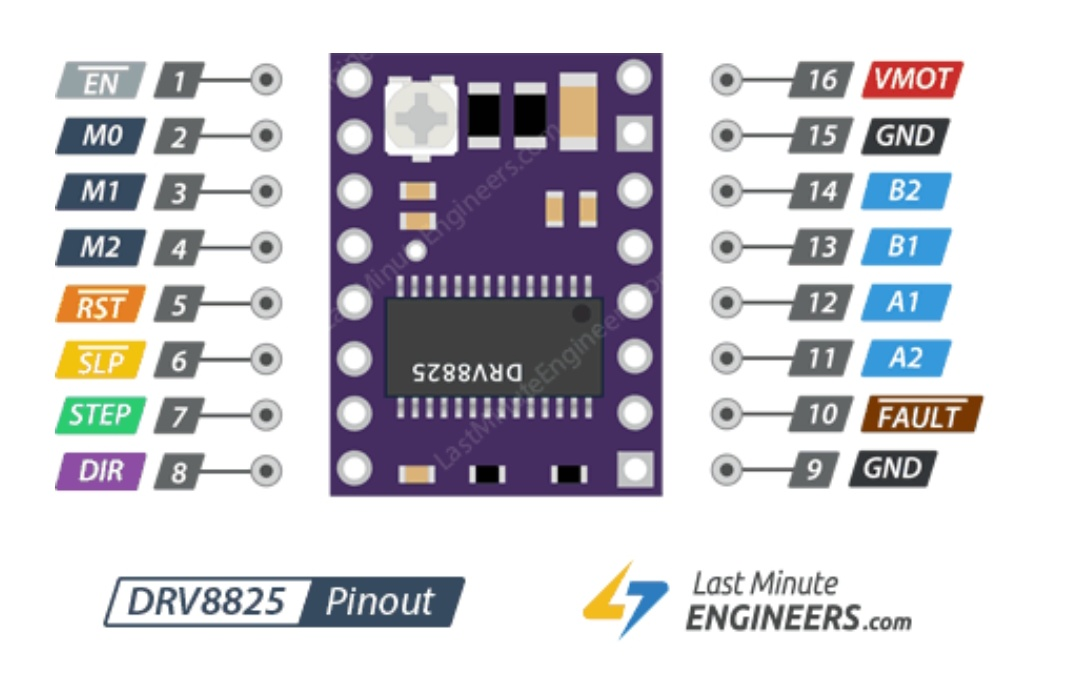
\includegraphics[width=0.6\textwidth]{ss1.jpg}
    \captionof{figure}{DRV8825 Pinout}
\end{center}

\end{document}
